\documentclass{article}
\usepackage[utf8]{inputenc}
\usepackage[T1]{fontenc}
\usepackage[english]{babel}
\setlength{\parindent}{0pt}
\usepackage{hyperref}
\hypersetup{
    colorlinks=true,
    linkcolor=blue,
    filecolor=magenta,      
    urlcolor=cyan}
\usepackage{graphicx}
\graphicspath{ {./pic/} }
\usepackage{multicol}
\usepackage{lscape}

\usepackage{fourier,amssymb,microtype,amsmath,gensymb}
\newcommand{\R}{\mathbb{R}}
\usepackage{mdframed,caption,xcolor}
\usepackage{tikz,tkz-euclide}

\title{Seminar 8. Mixed Strategies and Repeated Games}
\author{Xiaoguang Ling \\  \href{xiaoguang.ling@econ.uio.no}{xiaoguang.ling@econ.uio.no}}
\date{\today}

\begin{document}

\maketitle

%%%%%%%%%%%%%%%%%%%%%%%%%%%%%%%%%%%%%%%%%%%%%%%%%%%%%%%%%%%%%%%%%%%%%%%%%%%%%%%%%%%%%%%%%%%%%%

\section{Problem 1 - BR and UD} 

For each of the statements, if true, try to explain why, and if false, provide a
counter-example.

\bigskip

(a) In a finite normal-form game, if a pure strategy of a
player is not a best response to any belief that the player has about the strategies played by his opponents, then this pure strategy is strictly dominated by another \textit{pure} strategy.\\

\medskip

False. Consider:

\begin{center}
\captionof{table}{BR and UD for a 2-player normal form game}
\label{tab:brud}
\begin{tabular}{cc|c|c|}
  & \multicolumn{1}{c}{} & \multicolumn{2}{c}{$P2$}  \\
  & \multicolumn{1}{c}{} & \multicolumn{1}{c}{$d$} & \multicolumn{1}{c}{$e$} \\\cline{3-4}
            & $a$ & $(3,-)$ & $(0,-)$ \\   \cline{3-4}  
   $P1$ & $b$ & $(0,-)$ & $(3,-)$ \\   \cline{3-4}
            & $c$ & $(1,-)$ & $(1,-)$ \\   \cline{3-4}

\end{tabular}
\end{center}

The pure strategy $c$ is not a best response to any belief about $d$ and $e$.

\smallskip

\begin{mdframed}[backgroundcolor=blue!20,linecolor=white]
The correct statement is (Watson pp.58):

\begin{itemize}
\item In a finite two-player game,$B_1 = UD_1$ and $B_2 = UD_2$
\item For any finite game, $B_i \subset UD_i$ and $B^C_i = UD_i$ for $i = 1, 2,\cdots, n$.
\end{itemize}

Procedure for calculating $B_i$ (also $UD_i$) for two-player matrix games:

\begin{enumerate}
\item Look for strategies that are best responses to the simplest beliefs -- those beliefs that put all probability on just one of the other player's strategies.These best responses are obviously in the set $B_i$ so they are also in $UD_i$ .
\item Look for strategies that are dominated by other pure strategies; these dominated strategies are not in $UD_i$ and thus they are also not in $B_i$.
\item Test each remaining strategy to see if it is dominated by a mixed strategy. This final step is the most difficult, but if you are lucky, then you will rarely have to perform it.

\end{enumerate}

Let's look for $BR_1$ (which is also $UD_1$) in Table \ref{tab:brud}.

\begin{enumerate}
\item $BR_1(d)=a$, $BR_1(e)=b$, thus ${a,b}$ are obviously in the set $B_i$ (and $UD_i$).
\item ${c}$ is not dominated by any other pure strategies.
\item Can ${c}$ be dominated by a mixed strategy of $a,b$? Yes, for example, a mix strategy between ${a,b}$ with probability $(0.5,0.5)$ yeilds expected payoff $(1.5,1.5)$
\end{enumerate}

More precisely, let $q$ be the probability assigned to $a$ and $1-q$ the probability assigned to $b$.If ${c}$ is dominated by a mixed strategy of $d$ and $e$, we must have:

$$q\times 3 + (1-q)\times 0 > 1 \Rightarrow q > \tfrac13 $$
$$q\times 0 + (1-q)\times 3 >1 \Rightarrow p < \tfrac23 $$

That is, if $q\in (\tfrac13,\tfrac23)$, ${c}$ is dominated by a mixed strategy of $a$ and $b$.

\end{mdframed}


%
(b) In a finite normal-form game, if a pure strategy of a
player is not a best response to any belief that the player has about the strategies played by his opponents, then this pure strategy is strictly dominated by some \textit{mixed} strategy.

\medskip

True for a two-player game. In a finite two-player game,$B_1 = UD_1$ and $B_2 = UD_2$. A non-BR must not be UD either, thus it must be dominated by some strategy.


\begin{mdframed}[backgroundcolor=blue!20,linecolor=white]
It is outside the scope of this course to provide a formal proof of this result. In particular, in games with three or more player, the result requires that a player might have correlated beliefs about the strategies played by his opponents.

\smallskip

Read Watson pp.423 if you're interested in games with more than 2 players.
\end{mdframed}

%%%%%%%%%%%%%%%%%%%%%%%%%%%%%%%%%%%%%%%%%%%%%%%%%%%%%%%%%%%%%%%%%%%%%%%%%%%%%%%%%%%%%%%%%%%%%%
\newpage
\section{Problem 2 - Penalty kick} 

(Jehle and Reny pp.367, Problem 7.13)

Consider the penalty kick in soccer. There are two players, the goalie and the striker. 
\begin{itemize}
\item The striker has two strategies: kick to the goalie's right ($R$) or to the goalie's left ($L$). 
\item The goalie has two strategies: move left ($L$) or move right ($R$). 
\end{itemize}

Let $\alpha$ be the probability that the kick is stopped when both choose
L, and let $\beta$ be the probability that the kick is stopped when both choose $R$. 

Assume that $0 < \alpha < \beta < 1$. Consequently, the striker is more skilled at kicking to the goalie's left. The payoff matrix is as follows.

\begin{center}
{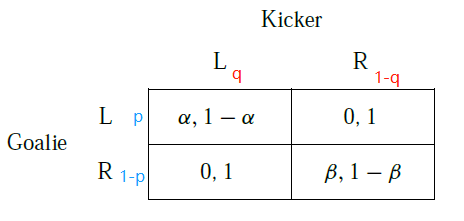
\includegraphics[width=0.5\textwidth]{8.q7_13}
\label{fig:q7_13}
\vspace{2mm}}
\end{center}


(a) Before analysing this game, informally answer the following questions.

\begin{itemize}
\item (i) Would you expect a striker who is more skilled at kicking to the goalie's left than to his
right, to score more often when he kicks to the goalie's left?
\item (ii) If a striker's ability to score when kicking to the goalie's left rises (i.e. $\alpha$ decreases) how will this affect the percentage of times the striker scores when he chooses to kick to the goalie's left? Will it affect his scoring percentage when he kicks right?

\end{itemize}



(b) Find the unique Nash equilibrium.

Both players choose $L$ with probability $\tfrac{\beta}{\alpha + \beta}$. To see this, let $p$ be the probability that the Goalie moves $L$ and $1-p$ the probability that the Golie moves $R$, and let $q$ be the probability that the Striker kicks $L$ and $1-q$ the probability that the Striker kicks $R$. This yields the following payoffs:
    \begin{itemize}
    \item If Goalie moves $L$: $q\alpha$.
    \item If Goalie moves $R$: $(1-q)\beta$.
    \item If Striker kicks $L$: $p(1-\alpha) + (1-p) = 1 - p\alpha$.
    \item If Striker kicks $R$: $p + (1-p)(1-\beta) = p + 1 - p - \beta + p\beta = 1 - (1-p)\beta$.
    \end{itemize}
    Thus, the Goalie is indifferent if $q\alpha = (1-q)\beta$. Therefore, $q$ must satisfy that $q(\alpha+\beta) = \beta$ or $q = \frac{\beta}{\alpha+\beta}$. And the Striker is indifferent if $p\alpha = (1-p)\beta$. Therefore, $p$ must satisfy that $p(\alpha+\beta) = \beta$ or $p = \frac{\beta}{\alpha+\beta}$.
    
(c) Answer again the questions in part (a). Based upon this, would it be wise to judge a striker's
relative scoring ability in kicking left versus right by comparing the fraction of times he scores
when he kicks right versus the fraction of times he scores when he kicks left?

\textit{(i) In the Nash equilibrium, the scoring probability is $1 - \tfrac{\alpha \beta}{\alpha + \beta}$ for both $L$ and $R$, since the goalie goes more often to the striker's good side. \\ (ii) When $\alpha$ decreases, the scoring probabilities for $L$ and $R$ are increased, but remain the same, equal to $1 - \tfrac{\alpha \beta}{\alpha + \beta}$. Therefore, it is not wise to judge a striker's relative scoring ability in kicking left versus right by comparing the fraction of times he scores when he kicks right versus the fraction of times he scores when he kicks left scoring ability.}

(d) Show that knowing the fraction of times a goal was scored when both players chose L and the
fraction of times a goal was scored when both players chose R would permit you to correctly
deduce the player's scoring ability when kicking left and right.

\textit{The probability of scoring if both choose $L$ is $1 – \alpha$, and the probability of scoring if both choose $R$ is $1 – \beta$. Since $1 – \alpha > 1 – \beta$, this shows correctly that the kicker is more skilled when choosing $L$.}

(e) Could you correctly deduce the player's scoring ability when kicking left and right if you only
had access to the striker's choice? If not, what can be deduced?

(f) Could you correctly deduce the player's scoring ability when kicking left versus right if you only
had access to the goalie's choice? If not, what can be deduced?




%%%%%%%%%%%%%%%%%%%%%%%%%%%%%%%%%%%%%%%%%%%%%%%%%%%%%%%%%%%%%%%%%%%%%%%%%%%%%%%%%%%%%%%%%%%%%%

\section{Problem 3} \textit{(Reporting a crime)}

A crime is observed by a group of $n$ people. Each person would like the police to be informed
but prefers that someone else make the phone call. Specifically, suppose that each person
attaches the value $v$ to the police being informed and bears the cost $c$ if she makes the
phone call, where $v > c > 0$.

\begin{itemize}
\item[(a)] Model this situation as normal form game. \textit{ \\ Players: $N = \{1, \dots , n \}$ \\ Strategy set for each player: $\{A, I \}$, where $A$: action and $I$: inaction \\ Payoff function: $0$ if self and others choose $I$; $v-c$ if self chooses $A$; $v$ is self chooses $I$ and some other chooses $A$.}
%
\item[(b)] Find the set of pure strategy Nash equilibria. \textit{ \\ $n$ different asymmetric pure strategy Nash equilibria where exactly one chooses $A$. (Why no incentive to deviate?) No symmetric pure strategy Nash equilibrium. (Why?)}
%
\item[(c)] Find the symmetric mixed strategy Nash equilibrium. \textit{ \\ In a mixed strategy mixed strategy Nash equilibrium, the players must be indifferent between $A$ and $I$:$$v-c = 0 \cdot \text{Prob}\{\text{no one else calls}\} + v \cdot \text{Prob}\{\text{at least one other calls}\} \, ,$$implying that $v-c = v \cdot (1 - \text{Prob}\{\text{no one else calls}\})$ so that $$\text{Prob}\{\text{no one else calls}\} = \tfrac{c}{v} \, .$$If we denote the probability of choosing $A$ by $p$, this implies$$\tfrac{c}{v} = (1-p)^{n-1} \quad \text{or} \quad p = 1 - \left( \tfrac{c}{v} \right)^\frac1{n-1} \, .$$ }
%
\item[(d)] In the symmetric mixed strategy Nash equilibrium, how does the probability that the
police will be called vary with the number of people $n$? \textit{ \\ The probability that no one calls is the product of the probability that one does not call ($1 - p = \left( \tfrac{c}{v} \right)^\frac1{n-1}$) and the probability that no one else calls ($\tfrac{c}{v}$). The latter does not vary with $n$, while the former increases with $n$. Therefore, the probability that no one calls increases with $n$, so that probability that someone calls decreases with $n$. This is one explanation of the so-called ``bystander effect''.}
%
\end{itemize}
\vspace{-6pt}


%%%%%%%%%%%%%%%%%%%%%%%%%%%%%%%%%%%%%%%%%%%%%%%%%%%%%%%%%%%%%%%%%%%%%%%%%%%%%%%%%%%%%%%%%%%%%%

\section{Problem 4} \textit{(Finitely repeated game)}

Watson Exercise pp. Q22.4 

If its stage game has exactly one Nash equilibrium, how many subgame
perfect equilibria does a two-period, repeated game have? Explain. Would
your answer change if there were T periods, where T is any finite integer?



In period 2, subgame perfection requires play of the only Nash equilibrium
of the stage game. As there is only one Nash equilibrium of the stage game,
selection of the Nash equilibrium to be played in period 2 cannot influence
incentives in period 1. Thus, the only subgame perfect equilibrium is play
of the Nash equilibrium of the stage game in both periods. For any finite
T, the logic from the two-period case applies, and the answer does not
change.


%%%%%%%%%%%%%%%%%%%%%%%%%%%%%%%%%%%%%%%%%%%%%%%%%%%%%%%%%%%%%%%%%%%%%%%%%%%%%%%%%%%%%%%%%%%%%%

\section{Problem 5} \textit{(Infinitely repeated game)}

Consider the following normal form game.

\begin{center}
$
\begin{array}{c|c|c|c|}
& L & C & R \\
\hline
U & 1,1 & 4,0 & 5,0 \\
\hline
M & 0,4 & 3,3 & 6,2 \\
\hline
D & 0,5 & 2,6 & 5,5 \\
\hline\end{array}
$
\end{center}

Assume now that this game is repeated infinitely many times. Assume furthermore that the players in each round can observe choices made in earlier rounds and that their payoff is the sum of payoffs discounted by the discount factor   $\delta$ (where $0 < \delta < 1$). Show that there exists a subgame perfect Nash equilibrium leading to the outcome path
$$(D, R), (D, R), (D, R), (D, R), \dots $$
if $\delta \geq 1/5$. \\ \textit{Consider the strategy profile determined by player 1 beginning with $D$ and player 2 with $R$ and that both player continue with this as long as only $D$ and $R$ have been played before. If not, player 1 plays $U$ and player 2 plays $L$. Deviating yields a short-run gain of $1$ and perpetual future loss of $4$. The present value of the short-run gain does not exceed the present value of the perpetual future loss if $\delta \geq \tfrac15$.}




\section{Problem 6} \textit{(Infinitely repeated price competition)}

Watson pp.318 Exercise 23.1, 


Consider the Bertrand oligopoly model, where $n$ firms simultaneously and independently
select their prices, $p_1 , p_2 , \cdots , p_n$ , in a market. (These prices are
greater than or equal to $0$.) Consumers observe these prices and only purchase
from the firm (or firms) with the lowest price $p$, according to the demand
curve $Q = 110 − p$, where $p = min{p_1 , p_2 , \cdots , p_n}$. That is, the firm with
the lowest price gets all of the sales. If the lowest price is offered by more than
one firm, then these firms equally share the quantity demanded $Q$. Assume
that firms must supply the quantities demanded of them and that production
takes place at a constant cost of $10$ per unit. (That is, the cost function for each
firm is $c (q) = 10q)$. Determining the Nash equilibrium of this game was the
subject of a previous exercise.






with the following additional question, to be answered before part (a):

What is the lowest price $\underline{p}$ in a Nash equilibrium if the game is played only once?
And what is the profits of the firms in a Nash equilibrium in this case? \\ \textit{In a Nash equilibrium at least two firms $i$ set $p_i = 10$ and that is minimum price. For the rest, see Watson, p.~464.}

(a) Suppose that this game is infinitely repeated. (The firms play the
game each period, for an infinite number of periods.) Define $\delta$  as the
discount factor for the firms. Imagine that the firms wish to sustain
a collusive arrangement in which they all select the monopoly price
$p^M = 60$ each period. What strategies might support this behavior in
equilibrium? (Do not solve for conditions under which equilibrium
occurs. Just explain what the strategies are. Remember, this requires
specifying how the firms punish each other. Use the Nash equilibrium
price as punishment.)

(b) Derive a condition on $n$ and $\delta$ that guarantees that collusion can be
sustained.

(c) What does your answer to part (b) imply about the optimal size of
cartels?


\end{document}
